\documentclass[twoside]{book}

% Packages required by doxygen
\usepackage{fixltx2e}
\usepackage{calc}
\usepackage{doxygen}
\usepackage[export]{adjustbox} % also loads graphicx
\usepackage{graphicx}
\usepackage[utf8]{inputenc}
\usepackage{makeidx}
\usepackage{multicol}
\usepackage{multirow}
\PassOptionsToPackage{warn}{textcomp}
\usepackage{textcomp}
\usepackage[nointegrals]{wasysym}
\usepackage[table]{xcolor}

% Font selection
\usepackage[T1]{fontenc}
\usepackage[scaled=.90]{helvet}
\usepackage{courier}
\usepackage{amssymb}
\usepackage{sectsty}
\renewcommand{\familydefault}{\sfdefault}
\allsectionsfont{%
  \fontseries{bc}\selectfont%
  \color{darkgray}%
}
\renewcommand{\DoxyLabelFont}{%
  \fontseries{bc}\selectfont%
  \color{darkgray}%
}
\newcommand{\+}{\discretionary{\mbox{\scriptsize$\hookleftarrow$}}{}{}}

% Page & text layout
\usepackage{geometry}
\geometry{%
  a4paper,%
  top=2.5cm,%
  bottom=2.5cm,%
  left=2.5cm,%
  right=2.5cm%
}
\tolerance=750
\hfuzz=15pt
\hbadness=750
\setlength{\emergencystretch}{15pt}
\setlength{\parindent}{0cm}
\setlength{\parskip}{3ex plus 2ex minus 2ex}
\makeatletter
\renewcommand{\paragraph}{%
  \@startsection{paragraph}{4}{0ex}{-1.0ex}{1.0ex}{%
    \normalfont\normalsize\bfseries\SS@parafont%
  }%
}
\renewcommand{\subparagraph}{%
  \@startsection{subparagraph}{5}{0ex}{-1.0ex}{1.0ex}{%
    \normalfont\normalsize\bfseries\SS@subparafont%
  }%
}
\makeatother

% Headers & footers
\usepackage{fancyhdr}
\pagestyle{fancyplain}
\fancyhead[LE]{\fancyplain{}{\bfseries\thepage}}
\fancyhead[CE]{\fancyplain{}{}}
\fancyhead[RE]{\fancyplain{}{\bfseries\leftmark}}
\fancyhead[LO]{\fancyplain{}{\bfseries\rightmark}}
\fancyhead[CO]{\fancyplain{}{}}
\fancyhead[RO]{\fancyplain{}{\bfseries\thepage}}
\fancyfoot[LE]{\fancyplain{}{}}
\fancyfoot[CE]{\fancyplain{}{}}
\fancyfoot[RE]{\fancyplain{}{\bfseries\scriptsize Generated by Doxygen }}
\fancyfoot[LO]{\fancyplain{}{\bfseries\scriptsize Generated by Doxygen }}
\fancyfoot[CO]{\fancyplain{}{}}
\fancyfoot[RO]{\fancyplain{}{}}
\renewcommand{\footrulewidth}{0.4pt}
\renewcommand{\chaptermark}[1]{%
  \markboth{#1}{}%
}
\renewcommand{\sectionmark}[1]{%
  \markright{\thesection\ #1}%
}

% Indices & bibliography
\usepackage{natbib}
\usepackage[titles]{tocloft}
\setcounter{tocdepth}{3}
\setcounter{secnumdepth}{5}
\makeindex

% Hyperlinks (required, but should be loaded last)
\usepackage{ifpdf}
\ifpdf
  \usepackage[pdftex,pagebackref=true]{hyperref}
\else
  \usepackage[ps2pdf,pagebackref=true]{hyperref}
\fi
\hypersetup{%
  colorlinks=true,%
  linkcolor=blue,%
  citecolor=blue,%
  unicode%
}

% Custom commands
\newcommand{\clearemptydoublepage}{%
  \newpage{\pagestyle{empty}\cleardoublepage}%
}

\usepackage{caption}
\captionsetup{labelsep=space,justification=centering,font={bf},singlelinecheck=off,skip=4pt,position=top}

%===== C O N T E N T S =====

\begin{document}

% Titlepage & ToC
\hypersetup{pageanchor=false,
             bookmarksnumbered=true,
             pdfencoding=unicode
            }
\pagenumbering{alph}
\begin{titlepage}
\vspace*{7cm}
\begin{center}%
{\Large Casse-\/\+Brique \\[1ex]\large 1.\+0 }\\
\vspace*{1cm}
{\large Generated by Doxygen 1.8.14}\\
\end{center}
\end{titlepage}
\clearemptydoublepage
\pagenumbering{roman}
\tableofcontents
\clearemptydoublepage
\pagenumbering{arabic}
\hypersetup{pageanchor=true}

%--- Begin generated contents ---
\chapter{Hierarchical Index}
\section{Class Hierarchy}
This inheritance list is sorted roughly, but not completely, alphabetically\+:\begin{DoxyCompactList}
\item \contentsline{section}{Ball}{\pageref{class_ball}}{}
\item \contentsline{section}{Game\+Manager}{\pageref{class_game_manager}}{}
\item list\begin{DoxyCompactList}
\item \contentsline{section}{List\+Player}{\pageref{class_list_player}}{}
\end{DoxyCompactList}
\item \contentsline{section}{Open\+Cv\+Widget}{\pageref{class_open_cv_widget}}{}
\item \contentsline{section}{Player}{\pageref{class_player}}{}
\item Q\+G\+L\+Widget\begin{DoxyCompactList}
\item \contentsline{section}{My\+G\+L\+Widget}{\pageref{class_my_g_l_widget}}{}
\end{DoxyCompactList}
\item Q\+Main\+Window\begin{DoxyCompactList}
\item \contentsline{section}{Main\+Window}{\pageref{class_main_window}}{}
\end{DoxyCompactList}
\item \contentsline{section}{Square}{\pageref{class_square}}{}
\begin{DoxyCompactList}
\item \contentsline{section}{Palette}{\pageref{class_palette}}{}
\end{DoxyCompactList}
\end{DoxyCompactList}

\chapter{Class Index}
\section{Class List}
Here are the classes, structs, unions and interfaces with brief descriptions\+:\begin{DoxyCompactList}
\item\contentsline{section}{\mbox{\hyperlink{class_ball}{Ball}} }{\pageref{class_ball}}{}
\item\contentsline{section}{\mbox{\hyperlink{class_game_manager}{Game\+Manager}} \\*Classe regroupant et gérant les éléments du jeu }{\pageref{class_game_manager}}{}
\item\contentsline{section}{\mbox{\hyperlink{class_list_player}{List\+Player}} }{\pageref{class_list_player}}{}
\item\contentsline{section}{\mbox{\hyperlink{class_main_window}{Main\+Window}} }{\pageref{class_main_window}}{}
\item\contentsline{section}{\mbox{\hyperlink{class_my_g_l_widget}{My\+G\+L\+Widget}} }{\pageref{class_my_g_l_widget}}{}
\item\contentsline{section}{\mbox{\hyperlink{class_open_cv_widget}{Open\+Cv\+Widget}} }{\pageref{class_open_cv_widget}}{}
\item\contentsline{section}{\mbox{\hyperlink{class_palette}{Palette}} }{\pageref{class_palette}}{}
\item\contentsline{section}{\mbox{\hyperlink{class_player}{Player}} }{\pageref{class_player}}{}
\item\contentsline{section}{\mbox{\hyperlink{class_square}{Square}} }{\pageref{class_square}}{}
\end{DoxyCompactList}

\chapter{File Index}
\section{File List}
Here is a list of all documented files with brief descriptions\+:\begin{DoxyCompactList}
\item\contentsline{section}{D\+:/\+Travail\+Etudiant/fise2-\/sem2/\+Q\+T\+Creator/\+Developpement projet/\+Casse-\/\+Brique/\+Breakout/{\bfseries ball.\+h} }{\pageref{ball_8h}}{}
\item\contentsline{section}{D\+:/\+Travail\+Etudiant/fise2-\/sem2/\+Q\+T\+Creator/\+Developpement projet/\+Casse-\/\+Brique/\+Breakout/\mbox{\hyperlink{gamemanager_8h}{gamemanager.\+h}} \\*Gestionnaire de Jeu }{\pageref{gamemanager_8h}}{}
\item\contentsline{section}{D\+:/\+Travail\+Etudiant/fise2-\/sem2/\+Q\+T\+Creator/\+Developpement projet/\+Casse-\/\+Brique/\+Breakout/{\bfseries listplayer.\+h} }{\pageref{listplayer_8h}}{}
\item\contentsline{section}{D\+:/\+Travail\+Etudiant/fise2-\/sem2/\+Q\+T\+Creator/\+Developpement projet/\+Casse-\/\+Brique/\+Breakout/{\bfseries mainwindow.\+h} }{\pageref{mainwindow_8h}}{}
\item\contentsline{section}{D\+:/\+Travail\+Etudiant/fise2-\/sem2/\+Q\+T\+Creator/\+Developpement projet/\+Casse-\/\+Brique/\+Breakout/{\bfseries myglwidget.\+h} }{\pageref{myglwidget_8h}}{}
\item\contentsline{section}{D\+:/\+Travail\+Etudiant/fise2-\/sem2/\+Q\+T\+Creator/\+Developpement projet/\+Casse-\/\+Brique/\+Breakout/{\bfseries opencvwidget.\+h} }{\pageref{opencvwidget_8h}}{}
\item\contentsline{section}{D\+:/\+Travail\+Etudiant/fise2-\/sem2/\+Q\+T\+Creator/\+Developpement projet/\+Casse-\/\+Brique/\+Breakout/{\bfseries palette.\+h} }{\pageref{palette_8h}}{}
\item\contentsline{section}{D\+:/\+Travail\+Etudiant/fise2-\/sem2/\+Q\+T\+Creator/\+Developpement projet/\+Casse-\/\+Brique/\+Breakout/{\bfseries player.\+h} }{\pageref{player_8h}}{}
\item\contentsline{section}{D\+:/\+Travail\+Etudiant/fise2-\/sem2/\+Q\+T\+Creator/\+Developpement projet/\+Casse-\/\+Brique/\+Breakout/{\bfseries square.\+h} }{\pageref{square_8h}}{}
\end{DoxyCompactList}

\chapter{Class Documentation}
\hypertarget{class_ball}{}\section{Ball Class Reference}
\label{class_ball}\index{Ball@{Ball}}
\subsection*{Public Member Functions}
\begin{DoxyCompactItemize}
\item 
\mbox{\Hypertarget{class_ball_a522a66cf500f94275cceb49b1635e962}\label{class_ball_a522a66cf500f94275cceb49b1635e962}} 
{\bfseries Ball} (double radius, double x, double y, double z, double speed)
\item 
\mbox{\Hypertarget{class_ball_ae639c8f2030279739228019198021e99}\label{class_ball_ae639c8f2030279739228019198021e99}} 
void {\bfseries reinitialiser} (double x, double y, double z)
\item 
\mbox{\Hypertarget{class_ball_a5c1bcd887f634369ed2b205199c3323c}\label{class_ball_a5c1bcd887f634369ed2b205199c3323c}} 
double {\bfseries get\+Radius} ()
\item 
\mbox{\Hypertarget{class_ball_a0d566e6196748ba2ff4c48e42b0ca7b1}\label{class_ball_a0d566e6196748ba2ff4c48e42b0ca7b1}} 
double {\bfseries getspeed} ()
\item 
\mbox{\Hypertarget{class_ball_a6806cba5442118acd06f48fd02cdd5cc}\label{class_ball_a6806cba5442118acd06f48fd02cdd5cc}} 
double {\bfseries getX} ()
\item 
\mbox{\Hypertarget{class_ball_ac4e44551d59c3c09d28444b41e1c623b}\label{class_ball_ac4e44551d59c3c09d28444b41e1c623b}} 
double {\bfseries getY} ()
\item 
\mbox{\Hypertarget{class_ball_a44bd04f6ba99b9a43c94e83a0e209359}\label{class_ball_a44bd04f6ba99b9a43c94e83a0e209359}} 
double {\bfseries getZ} ()
\item 
\mbox{\Hypertarget{class_ball_ad791ba74a79741d4d66f0fff6c1367d1}\label{class_ball_ad791ba74a79741d4d66f0fff6c1367d1}} 
Q\+String {\bfseries get\+State} ()
\item 
\mbox{\Hypertarget{class_ball_a697519c70a27af56967b88a1c69bd92a}\label{class_ball_a697519c70a27af56967b88a1c69bd92a}} 
void {\bfseries set\+State} (Q\+String change)
\item 
\mbox{\Hypertarget{class_ball_af17cd3a404b572e9a87e7589ea7bd8f7}\label{class_ball_af17cd3a404b572e9a87e7589ea7bd8f7}} 
double $\ast$ {\bfseries get\+Direction} ()
\item 
\mbox{\Hypertarget{class_ball_a3b36da76a1ea6c1e30ffa4ed60ccd446}\label{class_ball_a3b36da76a1ea6c1e30ffa4ed60ccd446}} 
double {\bfseries get\+DirectionX} ()
\item 
\mbox{\Hypertarget{class_ball_a791c67c6112d626112b09e43420089a6}\label{class_ball_a791c67c6112d626112b09e43420089a6}} 
double {\bfseries get\+DirectionY} ()
\item 
\mbox{\Hypertarget{class_ball_a7d6e946cfe6310088e938258cb9e88f1}\label{class_ball_a7d6e946cfe6310088e938258cb9e88f1}} 
double {\bfseries get\+DirectionZ} ()
\item 
\mbox{\Hypertarget{class_ball_a51f2f0f1e6aa3b1cee878c1713f31fbb}\label{class_ball_a51f2f0f1e6aa3b1cee878c1713f31fbb}} 
void {\bfseries set\+DirectionX} (double directionX)
\item 
\mbox{\Hypertarget{class_ball_a7758c0e5b90900b8984e602797798d12}\label{class_ball_a7758c0e5b90900b8984e602797798d12}} 
void {\bfseries set\+DirectionY} (double directionY)
\item 
\mbox{\Hypertarget{class_ball_a1f44da15c5d258b37d7e349f04e78890}\label{class_ball_a1f44da15c5d258b37d7e349f04e78890}} 
void {\bfseries set\+DirectionZ} (double directionZ)
\item 
\mbox{\Hypertarget{class_ball_a67a08cf9315f3f2c38408f0f24ffd389}\label{class_ball_a67a08cf9315f3f2c38408f0f24ffd389}} 
void {\bfseries setX} (double X)
\item 
\mbox{\Hypertarget{class_ball_a074c539ee788dda3edcd3dbafe46c6b1}\label{class_ball_a074c539ee788dda3edcd3dbafe46c6b1}} 
void {\bfseries setY} (double Y)
\item 
\mbox{\Hypertarget{class_ball_ae58e925566371743c7fe20af87d007f9}\label{class_ball_ae58e925566371743c7fe20af87d007f9}} 
void {\bfseries setZ} (double Z)
\item 
\mbox{\Hypertarget{class_ball_a991945691ac284db8cdd5b216f7f8223}\label{class_ball_a991945691ac284db8cdd5b216f7f8223}} 
void {\bfseries set\+Radius} (double radius)
\item 
\mbox{\Hypertarget{class_ball_acf8c22e5244ca7ab3d1d7af9aa6f3f18}\label{class_ball_acf8c22e5244ca7ab3d1d7af9aa6f3f18}} 
void {\bfseries set\+Speed} (double speed)
\end{DoxyCompactItemize}


The documentation for this class was generated from the following files\+:\begin{DoxyCompactItemize}
\item 
D\+:/\+Travail\+Etudiant/fise2-\/sem2/\+Q\+T\+Creator/\+Developpement projet/\+Casse-\/\+Brique/\+Breakout/ball.\+h\item 
D\+:/\+Travail\+Etudiant/fise2-\/sem2/\+Q\+T\+Creator/\+Developpement projet/\+Casse-\/\+Brique/\+Breakout/ball.\+cpp\end{DoxyCompactItemize}

\hypertarget{class_game_manager}{}\section{Game\+Manager Class Reference}
\label{class_game_manager}\index{Game\+Manager@{Game\+Manager}}


Classe regroupant et gérant les éléments du jeu.  


\subsection*{Public Member Functions}
\begin{DoxyCompactItemize}
\item 
\mbox{\hyperlink{class_game_manager_aa0e2424dc1a39d380e5b6605b179bf05}{Game\+Manager}} ()
\begin{DoxyCompactList}\small\item\em Constructeur. \end{DoxyCompactList}\item 
void \mbox{\hyperlink{class_game_manager_a707019231d8892afbe87da17dc31ae9e}{change\+Mode}} ()
\begin{DoxyCompactList}\small\item\em change\+Mode \end{DoxyCompactList}\item 
void \mbox{\hyperlink{class_game_manager_a982951601283ec375c115cd3f19b64a2}{reinitialiser\+Bricks}} ()
\begin{DoxyCompactList}\small\item\em reinitialiser\+Bricks \end{DoxyCompactList}\item 
void \mbox{\hyperlink{class_game_manager_aec56f391111fb15f43711719da20e407}{initialize\+Nb\+Win}} ()
\begin{DoxyCompactList}\small\item\em initialize\+Nb\+Win \end{DoxyCompactList}\item 
int \mbox{\hyperlink{class_game_manager_a2bd2b0363ac1c5c6026029fba4d41e38}{collision\+Brick}} (\mbox{\hyperlink{class_square}{Square}} brick)
\begin{DoxyCompactList}\small\item\em collision\+Brick \end{DoxyCompactList}\item 
int \mbox{\hyperlink{class_game_manager_aaab1c8649edbdc0496371a83bad05cb4}{collision\+Wall}} (double dimension\+Max, double width, double height)
\begin{DoxyCompactList}\small\item\em collision\+Wall \end{DoxyCompactList}\item 
\mbox{\Hypertarget{class_game_manager_af72705118801e4011c3343ac9a8b5335}\label{class_game_manager_af72705118801e4011c3343ac9a8b5335}} 
void \mbox{\hyperlink{class_game_manager_af72705118801e4011c3343ac9a8b5335}{update\+Bille\+\_\+\+Score}} ()
\begin{DoxyCompactList}\small\item\em update\+Bille\+\_\+\+Score Met à jour Position de la Bille,la Vie des briques et le score du joueur en fonction de l\textquotesingle{}état de la liste de brick \end{DoxyCompactList}\item 
void \mbox{\hyperlink{class_game_manager_a10193620d465e7e17285be2533e03f78}{update\+Nb\+Win}} ()
\begin{DoxyCompactList}\small\item\em update\+Nb\+Win \end{DoxyCompactList}\item 
void \mbox{\hyperlink{class_game_manager_aba55e5cb8867a408fc2492d732446ab8}{update\+Position\+Palette}} ()
\begin{DoxyCompactList}\small\item\em update\+Position\+Palette \end{DoxyCompactList}\item 
double \mbox{\hyperlink{class_game_manager_ab6b2748c5280bc20cbed15f32a18deb9}{search\+Position\+Impact}} (\mbox{\hyperlink{class_palette}{Palette}} brick)
\begin{DoxyCompactList}\small\item\em search\+Position\+Impact Cherche la position de l\textquotesingle{}impact entre la bille et la palette \end{DoxyCompactList}\item 
\mbox{\hyperlink{class_ball}{Ball}} \mbox{\hyperlink{class_game_manager_af7c8890b2880ac4a7e9df9b5359d0392}{get\+Bille}} ()
\begin{DoxyCompactList}\small\item\em get\+Bille \end{DoxyCompactList}\item 
\mbox{\hyperlink{class_palette}{Palette}} \mbox{\hyperlink{class_game_manager_ae28734a8c38cffbd7fc2ab4f8a996543}{get\+Stick}} ()
\begin{DoxyCompactList}\small\item\em get\+Stick \end{DoxyCompactList}\item 
\mbox{\hyperlink{class_player}{Player}} \mbox{\hyperlink{class_game_manager_aebb883b6b25f5e017d315f692d5cd5a1}{get\+Player}} ()
\begin{DoxyCompactList}\small\item\em get\+Player \end{DoxyCompactList}\item 
int \mbox{\hyperlink{class_game_manager_a8b770addd88c3e9dba5691e38ec59a2b}{get\+Nb\+Win}} ()
\begin{DoxyCompactList}\small\item\em get\+Nb\+Win \end{DoxyCompactList}\item 
Q\+String \mbox{\hyperlink{class_game_manager_a0eb6a90c2608f741f37d870a7b90255c}{get\+State}} ()
\begin{DoxyCompactList}\small\item\em get\+State \end{DoxyCompactList}\item 
\mbox{\hyperlink{class_square}{Square}} \mbox{\hyperlink{class_game_manager_ac3efa1f197bd8d0869b41bd969e02fd0}{get\+BrickI}} (int i)
\begin{DoxyCompactList}\small\item\em get\+BrickI \end{DoxyCompactList}\end{DoxyCompactItemize}
\subsection*{Public Attributes}
\begin{DoxyCompactItemize}
\item 
\mbox{\hyperlink{class_ball}{Ball}} \mbox{\hyperlink{class_game_manager_a3c6413d0d78b839784ed4960d82d8501}{bille\+\_\+}}
\item 
\mbox{\hyperlink{class_square}{Square}} \mbox{\hyperlink{class_game_manager_a1f4d4e5f73f424ba4d04492e2b38cb88}{listbricks\+\_\+}} \mbox{[}70\mbox{]}
\item 
\mbox{\hyperlink{class_palette}{Palette}} \mbox{\hyperlink{class_game_manager_a086b81b6572ee3e4505143e284c2d503}{stick\+\_\+}}
\item 
\mbox{\hyperlink{class_player}{Player}} \mbox{\hyperlink{class_game_manager_af93b2a683a681a346d22577cd75a9dd5}{player}}
\item 
Q\+String \mbox{\hyperlink{class_game_manager_ade8777ca190763f4314035f7ee5905c2}{state\+\_\+}}
\item 
int \mbox{\hyperlink{class_game_manager_ac69eb2bd39346ff2c5304c6af93a6406}{nbwin\+\_\+}}
\item 
\mbox{\Hypertarget{class_game_manager_a04e5a46806b4c6199a688f1e91ff2d0f}\label{class_game_manager_a04e5a46806b4c6199a688f1e91ff2d0f}} 
bool {\bfseries mouse\+Event\+Act} =false
\end{DoxyCompactItemize}


\subsection{Detailed Description}
Classe regroupant et gérant les éléments du jeu. 

\subsection{Constructor \& Destructor Documentation}
\mbox{\Hypertarget{class_game_manager_aa0e2424dc1a39d380e5b6605b179bf05}\label{class_game_manager_aa0e2424dc1a39d380e5b6605b179bf05}} 
\index{Game\+Manager@{Game\+Manager}!Game\+Manager@{Game\+Manager}}
\index{Game\+Manager@{Game\+Manager}!Game\+Manager@{Game\+Manager}}
\subsubsection{\texorpdfstring{Game\+Manager()}{GameManager()}}
{\footnotesize\ttfamily Game\+Manager\+::\+Game\+Manager (\begin{DoxyParamCaption}{ }\end{DoxyParamCaption})}



Constructeur. 

Constructeur de la classe \mbox{\hyperlink{class_game_manager}{Game\+Manager}} 

\subsection{Member Function Documentation}
\mbox{\Hypertarget{class_game_manager_a707019231d8892afbe87da17dc31ae9e}\label{class_game_manager_a707019231d8892afbe87da17dc31ae9e}} 
\index{Game\+Manager@{Game\+Manager}!change\+Mode@{change\+Mode}}
\index{change\+Mode@{change\+Mode}!Game\+Manager@{Game\+Manager}}
\subsubsection{\texorpdfstring{change\+Mode()}{changeMode()}}
{\footnotesize\ttfamily void Game\+Manager\+::change\+Mode (\begin{DoxyParamCaption}{ }\end{DoxyParamCaption})\hspace{0.3cm}{\ttfamily [inline]}}



change\+Mode 

Changement du mode de Jeu (Mode souris ou caméra) \mbox{\Hypertarget{class_game_manager_a2bd2b0363ac1c5c6026029fba4d41e38}\label{class_game_manager_a2bd2b0363ac1c5c6026029fba4d41e38}} 
\index{Game\+Manager@{Game\+Manager}!collision\+Brick@{collision\+Brick}}
\index{collision\+Brick@{collision\+Brick}!Game\+Manager@{Game\+Manager}}
\subsubsection{\texorpdfstring{collision\+Brick()}{collisionBrick()}}
{\footnotesize\ttfamily int Game\+Manager\+::collision\+Brick (\begin{DoxyParamCaption}\item[{\mbox{\hyperlink{class_square}{Square}}}]{brick }\end{DoxyParamCaption})}



collision\+Brick 

Detecte si il y a collision entre la bille et la brick


\begin{DoxyParams}{Parameters}
{\em brick} & \+:Brick sur laquelle on cherche à determiner si il y a collision \\
\hline
\end{DoxyParams}
\begin{DoxyReturn}{Returns}
\+:Renvoie un entier entre 0 et 8 indiquant la collision avec une brick et met à jour sa vie 
\end{DoxyReturn}
\mbox{\Hypertarget{class_game_manager_aaab1c8649edbdc0496371a83bad05cb4}\label{class_game_manager_aaab1c8649edbdc0496371a83bad05cb4}} 
\index{Game\+Manager@{Game\+Manager}!collision\+Wall@{collision\+Wall}}
\index{collision\+Wall@{collision\+Wall}!Game\+Manager@{Game\+Manager}}
\subsubsection{\texorpdfstring{collision\+Wall()}{collisionWall()}}
{\footnotesize\ttfamily int Game\+Manager\+::collision\+Wall (\begin{DoxyParamCaption}\item[{double}]{dimension\+Max,  }\item[{double}]{width,  }\item[{double}]{height }\end{DoxyParamCaption})}



collision\+Wall 

Detecte si il y a collision entre la bille et les murs


\begin{DoxyParams}{Parameters}
{\em dimension\+Max} & \+:Dimension Max du Plateau \\
\hline
{\em width} & \+:Largeur du plateau \\
\hline
{\em height} & \+:Hauteur du plateau \\
\hline
\end{DoxyParams}
\begin{DoxyReturn}{Returns}
Renvoie un entier entre 0 et 8 indiquant la collision avec les bords du plateau 
\end{DoxyReturn}
\mbox{\Hypertarget{class_game_manager_af7c8890b2880ac4a7e9df9b5359d0392}\label{class_game_manager_af7c8890b2880ac4a7e9df9b5359d0392}} 
\index{Game\+Manager@{Game\+Manager}!get\+Bille@{get\+Bille}}
\index{get\+Bille@{get\+Bille}!Game\+Manager@{Game\+Manager}}
\subsubsection{\texorpdfstring{get\+Bille()}{getBille()}}
{\footnotesize\ttfamily \mbox{\hyperlink{class_ball}{Ball}} Game\+Manager\+::get\+Bille (\begin{DoxyParamCaption}{ }\end{DoxyParamCaption})\hspace{0.3cm}{\ttfamily [inline]}}



get\+Bille 

\begin{DoxyReturn}{Returns}

\end{DoxyReturn}
\mbox{\Hypertarget{class_game_manager_ac3efa1f197bd8d0869b41bd969e02fd0}\label{class_game_manager_ac3efa1f197bd8d0869b41bd969e02fd0}} 
\index{Game\+Manager@{Game\+Manager}!get\+BrickI@{get\+BrickI}}
\index{get\+BrickI@{get\+BrickI}!Game\+Manager@{Game\+Manager}}
\subsubsection{\texorpdfstring{get\+Brick\+I()}{getBrickI()}}
{\footnotesize\ttfamily \mbox{\hyperlink{class_square}{Square}} Game\+Manager\+::get\+BrickI (\begin{DoxyParamCaption}\item[{int}]{i }\end{DoxyParamCaption})\hspace{0.3cm}{\ttfamily [inline]}}



get\+BrickI 


\begin{DoxyParams}{Parameters}
{\em i\+:numéro} & de la brick que l\textquotesingle{}on souhaite obtenir \\
\hline
\end{DoxyParams}
\begin{DoxyReturn}{Returns}
Brick numéro i de listbricks 
\end{DoxyReturn}
\mbox{\Hypertarget{class_game_manager_a8b770addd88c3e9dba5691e38ec59a2b}\label{class_game_manager_a8b770addd88c3e9dba5691e38ec59a2b}} 
\index{Game\+Manager@{Game\+Manager}!get\+Nb\+Win@{get\+Nb\+Win}}
\index{get\+Nb\+Win@{get\+Nb\+Win}!Game\+Manager@{Game\+Manager}}
\subsubsection{\texorpdfstring{get\+Nb\+Win()}{getNbWin()}}
{\footnotesize\ttfamily int Game\+Manager\+::get\+Nb\+Win (\begin{DoxyParamCaption}{ }\end{DoxyParamCaption})\hspace{0.3cm}{\ttfamily [inline]}}



get\+Nb\+Win 

\begin{DoxyReturn}{Returns}

\end{DoxyReturn}
\mbox{\Hypertarget{class_game_manager_aebb883b6b25f5e017d315f692d5cd5a1}\label{class_game_manager_aebb883b6b25f5e017d315f692d5cd5a1}} 
\index{Game\+Manager@{Game\+Manager}!get\+Player@{get\+Player}}
\index{get\+Player@{get\+Player}!Game\+Manager@{Game\+Manager}}
\subsubsection{\texorpdfstring{get\+Player()}{getPlayer()}}
{\footnotesize\ttfamily \mbox{\hyperlink{class_player}{Player}} Game\+Manager\+::get\+Player (\begin{DoxyParamCaption}{ }\end{DoxyParamCaption})\hspace{0.3cm}{\ttfamily [inline]}}



get\+Player 

\begin{DoxyReturn}{Returns}

\end{DoxyReturn}
\mbox{\Hypertarget{class_game_manager_a0eb6a90c2608f741f37d870a7b90255c}\label{class_game_manager_a0eb6a90c2608f741f37d870a7b90255c}} 
\index{Game\+Manager@{Game\+Manager}!get\+State@{get\+State}}
\index{get\+State@{get\+State}!Game\+Manager@{Game\+Manager}}
\subsubsection{\texorpdfstring{get\+State()}{getState()}}
{\footnotesize\ttfamily Q\+String Game\+Manager\+::get\+State (\begin{DoxyParamCaption}{ }\end{DoxyParamCaption})\hspace{0.3cm}{\ttfamily [inline]}}



get\+State 

\begin{DoxyReturn}{Returns}

\end{DoxyReturn}
\mbox{\Hypertarget{class_game_manager_ae28734a8c38cffbd7fc2ab4f8a996543}\label{class_game_manager_ae28734a8c38cffbd7fc2ab4f8a996543}} 
\index{Game\+Manager@{Game\+Manager}!get\+Stick@{get\+Stick}}
\index{get\+Stick@{get\+Stick}!Game\+Manager@{Game\+Manager}}
\subsubsection{\texorpdfstring{get\+Stick()}{getStick()}}
{\footnotesize\ttfamily \mbox{\hyperlink{class_palette}{Palette}} Game\+Manager\+::get\+Stick (\begin{DoxyParamCaption}{ }\end{DoxyParamCaption})\hspace{0.3cm}{\ttfamily [inline]}}



get\+Stick 

\begin{DoxyReturn}{Returns}

\end{DoxyReturn}
\mbox{\Hypertarget{class_game_manager_aec56f391111fb15f43711719da20e407}\label{class_game_manager_aec56f391111fb15f43711719da20e407}} 
\index{Game\+Manager@{Game\+Manager}!initialize\+Nb\+Win@{initialize\+Nb\+Win}}
\index{initialize\+Nb\+Win@{initialize\+Nb\+Win}!Game\+Manager@{Game\+Manager}}
\subsubsection{\texorpdfstring{initialize\+Nb\+Win()}{initializeNbWin()}}
{\footnotesize\ttfamily void Game\+Manager\+::initialize\+Nb\+Win (\begin{DoxyParamCaption}{ }\end{DoxyParamCaption})\hspace{0.3cm}{\ttfamily [inline]}}



initialize\+Nb\+Win 

initialise la variable nbwin\+\_\+ \mbox{\Hypertarget{class_game_manager_a982951601283ec375c115cd3f19b64a2}\label{class_game_manager_a982951601283ec375c115cd3f19b64a2}} 
\index{Game\+Manager@{Game\+Manager}!reinitialiser\+Bricks@{reinitialiser\+Bricks}}
\index{reinitialiser\+Bricks@{reinitialiser\+Bricks}!Game\+Manager@{Game\+Manager}}
\subsubsection{\texorpdfstring{reinitialiser\+Bricks()}{reinitialiserBricks()}}
{\footnotesize\ttfamily void Game\+Manager\+::reinitialiser\+Bricks (\begin{DoxyParamCaption}{ }\end{DoxyParamCaption})}



reinitialiser\+Bricks 

Réinitialise la liste de brick en fonction du niveau de difficulté \mbox{\Hypertarget{class_game_manager_ab6b2748c5280bc20cbed15f32a18deb9}\label{class_game_manager_ab6b2748c5280bc20cbed15f32a18deb9}} 
\index{Game\+Manager@{Game\+Manager}!search\+Position\+Impact@{search\+Position\+Impact}}
\index{search\+Position\+Impact@{search\+Position\+Impact}!Game\+Manager@{Game\+Manager}}
\subsubsection{\texorpdfstring{search\+Position\+Impact()}{searchPositionImpact()}}
{\footnotesize\ttfamily double Game\+Manager\+::search\+Position\+Impact (\begin{DoxyParamCaption}\item[{\mbox{\hyperlink{class_palette}{Palette}}}]{brick }\end{DoxyParamCaption})}



search\+Position\+Impact Cherche la position de l\textquotesingle{}impact entre la bille et la palette 


\begin{DoxyParams}{Parameters}
{\em brick} & \+: \mbox{\hyperlink{class_palette}{Palette}} de jeu \\
\hline
\end{DoxyParams}
\begin{DoxyReturn}{Returns}
Position en X de l\textquotesingle{}impact 
\end{DoxyReturn}
\mbox{\Hypertarget{class_game_manager_a10193620d465e7e17285be2533e03f78}\label{class_game_manager_a10193620d465e7e17285be2533e03f78}} 
\index{Game\+Manager@{Game\+Manager}!update\+Nb\+Win@{update\+Nb\+Win}}
\index{update\+Nb\+Win@{update\+Nb\+Win}!Game\+Manager@{Game\+Manager}}
\subsubsection{\texorpdfstring{update\+Nb\+Win()}{updateNbWin()}}
{\footnotesize\ttfamily void Game\+Manager\+::update\+Nb\+Win (\begin{DoxyParamCaption}{ }\end{DoxyParamCaption})}



update\+Nb\+Win 

Met à jour le Level sur lequel on se situe et le comptage du nombre de victoire \mbox{\Hypertarget{class_game_manager_aba55e5cb8867a408fc2492d732446ab8}\label{class_game_manager_aba55e5cb8867a408fc2492d732446ab8}} 
\index{Game\+Manager@{Game\+Manager}!update\+Position\+Palette@{update\+Position\+Palette}}
\index{update\+Position\+Palette@{update\+Position\+Palette}!Game\+Manager@{Game\+Manager}}
\subsubsection{\texorpdfstring{update\+Position\+Palette()}{updatePositionPalette()}}
{\footnotesize\ttfamily void Game\+Manager\+::update\+Position\+Palette (\begin{DoxyParamCaption}{ }\end{DoxyParamCaption})}



update\+Position\+Palette 

Met à jour la position de la palette dans le mode Camera 

\subsection{Member Data Documentation}
\mbox{\Hypertarget{class_game_manager_a3c6413d0d78b839784ed4960d82d8501}\label{class_game_manager_a3c6413d0d78b839784ed4960d82d8501}} 
\index{Game\+Manager@{Game\+Manager}!bille\+\_\+@{bille\+\_\+}}
\index{bille\+\_\+@{bille\+\_\+}!Game\+Manager@{Game\+Manager}}
\subsubsection{\texorpdfstring{bille\+\_\+}{bille\_}}
{\footnotesize\ttfamily \mbox{\hyperlink{class_ball}{Ball}} Game\+Manager\+::bille\+\_\+}

Bille du jeu \mbox{\Hypertarget{class_game_manager_a1f4d4e5f73f424ba4d04492e2b38cb88}\label{class_game_manager_a1f4d4e5f73f424ba4d04492e2b38cb88}} 
\index{Game\+Manager@{Game\+Manager}!listbricks\+\_\+@{listbricks\+\_\+}}
\index{listbricks\+\_\+@{listbricks\+\_\+}!Game\+Manager@{Game\+Manager}}
\subsubsection{\texorpdfstring{listbricks\+\_\+}{listbricks\_}}
{\footnotesize\ttfamily \mbox{\hyperlink{class_square}{Square}} Game\+Manager\+::listbricks\+\_\+\mbox{[}70\mbox{]}}

Liste avec pour taille le nombre de lignes de bricks maximum $\ast$10 \mbox{\Hypertarget{class_game_manager_ac69eb2bd39346ff2c5304c6af93a6406}\label{class_game_manager_ac69eb2bd39346ff2c5304c6af93a6406}} 
\index{Game\+Manager@{Game\+Manager}!nbwin\+\_\+@{nbwin\+\_\+}}
\index{nbwin\+\_\+@{nbwin\+\_\+}!Game\+Manager@{Game\+Manager}}
\subsubsection{\texorpdfstring{nbwin\+\_\+}{nbwin\_}}
{\footnotesize\ttfamily int Game\+Manager\+::nbwin\+\_\+}

Niveau de difficulté du jeu \mbox{\Hypertarget{class_game_manager_af93b2a683a681a346d22577cd75a9dd5}\label{class_game_manager_af93b2a683a681a346d22577cd75a9dd5}} 
\index{Game\+Manager@{Game\+Manager}!player@{player}}
\index{player@{player}!Game\+Manager@{Game\+Manager}}
\subsubsection{\texorpdfstring{player}{player}}
{\footnotesize\ttfamily \mbox{\hyperlink{class_player}{Player}} Game\+Manager\+::player}

Joueur \mbox{\Hypertarget{class_game_manager_ade8777ca190763f4314035f7ee5905c2}\label{class_game_manager_ade8777ca190763f4314035f7ee5905c2}} 
\index{Game\+Manager@{Game\+Manager}!state\+\_\+@{state\+\_\+}}
\index{state\+\_\+@{state\+\_\+}!Game\+Manager@{Game\+Manager}}
\subsubsection{\texorpdfstring{state\+\_\+}{state\_}}
{\footnotesize\ttfamily Q\+String Game\+Manager\+::state\+\_\+}

Etats du jeu (peut prendre deux valeurs \mbox{\Hypertarget{class_game_manager_a086b81b6572ee3e4505143e284c2d503}\label{class_game_manager_a086b81b6572ee3e4505143e284c2d503}} 
\index{Game\+Manager@{Game\+Manager}!stick\+\_\+@{stick\+\_\+}}
\index{stick\+\_\+@{stick\+\_\+}!Game\+Manager@{Game\+Manager}}
\subsubsection{\texorpdfstring{stick\+\_\+}{stick\_}}
{\footnotesize\ttfamily \mbox{\hyperlink{class_palette}{Palette}} Game\+Manager\+::stick\+\_\+}

\mbox{\hyperlink{class_palette}{Palette}} du jeu permettant de renvoyer la balle et de la diriger 

The documentation for this class was generated from the following files\+:\begin{DoxyCompactItemize}
\item 
D\+:/\+Travail\+Etudiant/fise2-\/sem2/\+Q\+T\+Creator/\+Developpement projet/\+Casse-\/\+Brique/\+Breakout/\mbox{\hyperlink{gamemanager_8h}{gamemanager.\+h}}\item 
D\+:/\+Travail\+Etudiant/fise2-\/sem2/\+Q\+T\+Creator/\+Developpement projet/\+Casse-\/\+Brique/\+Breakout/gamemanager.\+cpp\end{DoxyCompactItemize}

\hypertarget{class_list_player}{}\section{List\+Player Class Reference}
\label{class_list_player}\index{List\+Player@{List\+Player}}
Inheritance diagram for List\+Player\+:\begin{figure}[H]
\begin{center}
\leavevmode
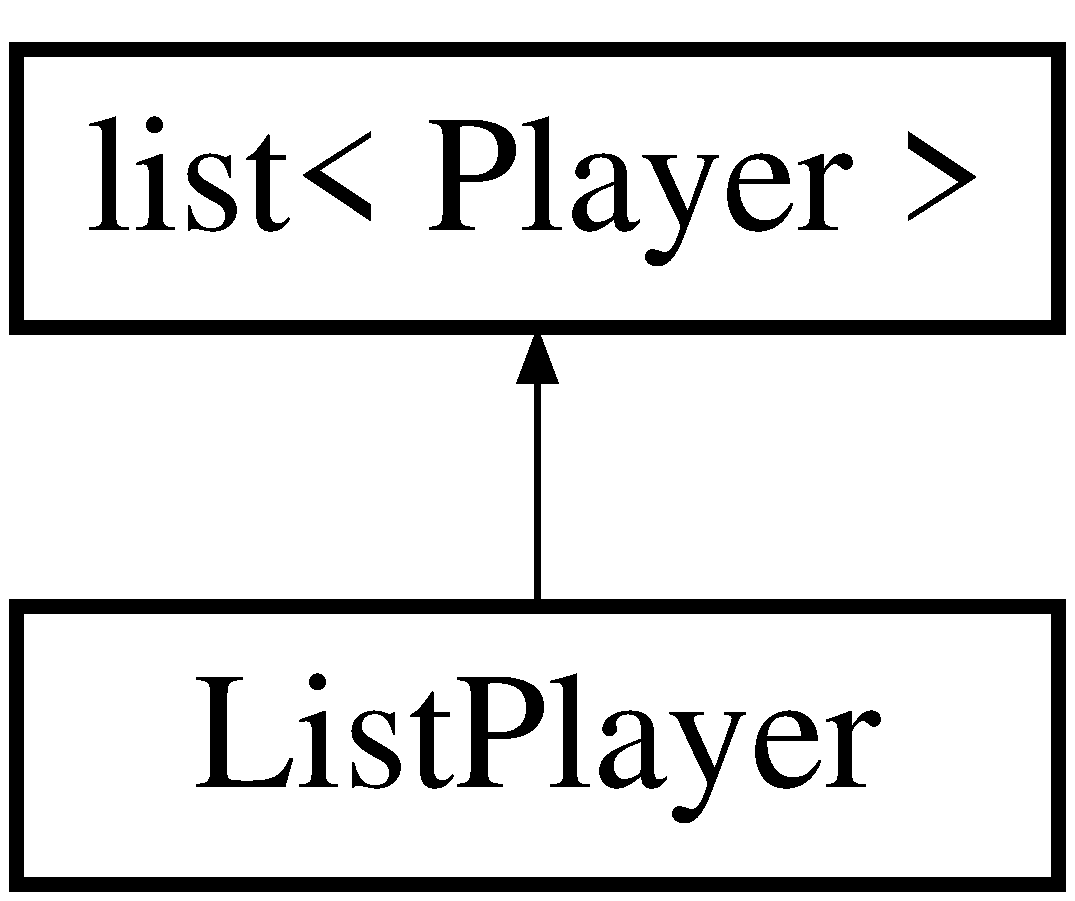
\includegraphics[height=2.000000cm]{class_list_player}
\end{center}
\end{figure}
\subsection*{Public Member Functions}
\begin{DoxyCompactItemize}
\item 
\mbox{\Hypertarget{class_list_player_a51419d9b0d08358b6384e13c462247b4}\label{class_list_player_a51419d9b0d08358b6384e13c462247b4}} 
void {\bfseries charger} (std\+::ifstream \&is)
\item 
\mbox{\Hypertarget{class_list_player_ad350875939b59a7a0203b7e7c4cc6602}\label{class_list_player_ad350875939b59a7a0203b7e7c4cc6602}} 
void {\bfseries sauver} (std\+::ofstream \&os)
\item 
\mbox{\Hypertarget{class_list_player_a5b8f02efc75e1bafd2300ac2d308eda5}\label{class_list_player_a5b8f02efc75e1bafd2300ac2d308eda5}} 
void {\bfseries tri\+List} ()
\end{DoxyCompactItemize}


The documentation for this class was generated from the following files\+:\begin{DoxyCompactItemize}
\item 
D\+:/\+Travail\+Etudiant/fise2-\/sem2/\+Q\+T\+Creator/\+Developpement projet/\+Casse-\/\+Brique/\+Breakout/listplayer.\+h\item 
D\+:/\+Travail\+Etudiant/fise2-\/sem2/\+Q\+T\+Creator/\+Developpement projet/\+Casse-\/\+Brique/\+Breakout/listplayer.\+cpp\end{DoxyCompactItemize}

\hypertarget{class_main_window}{}\section{Main\+Window Class Reference}
\label{class_main_window}\index{Main\+Window@{Main\+Window}}
Inheritance diagram for Main\+Window\+:\begin{figure}[H]
\begin{center}
\leavevmode
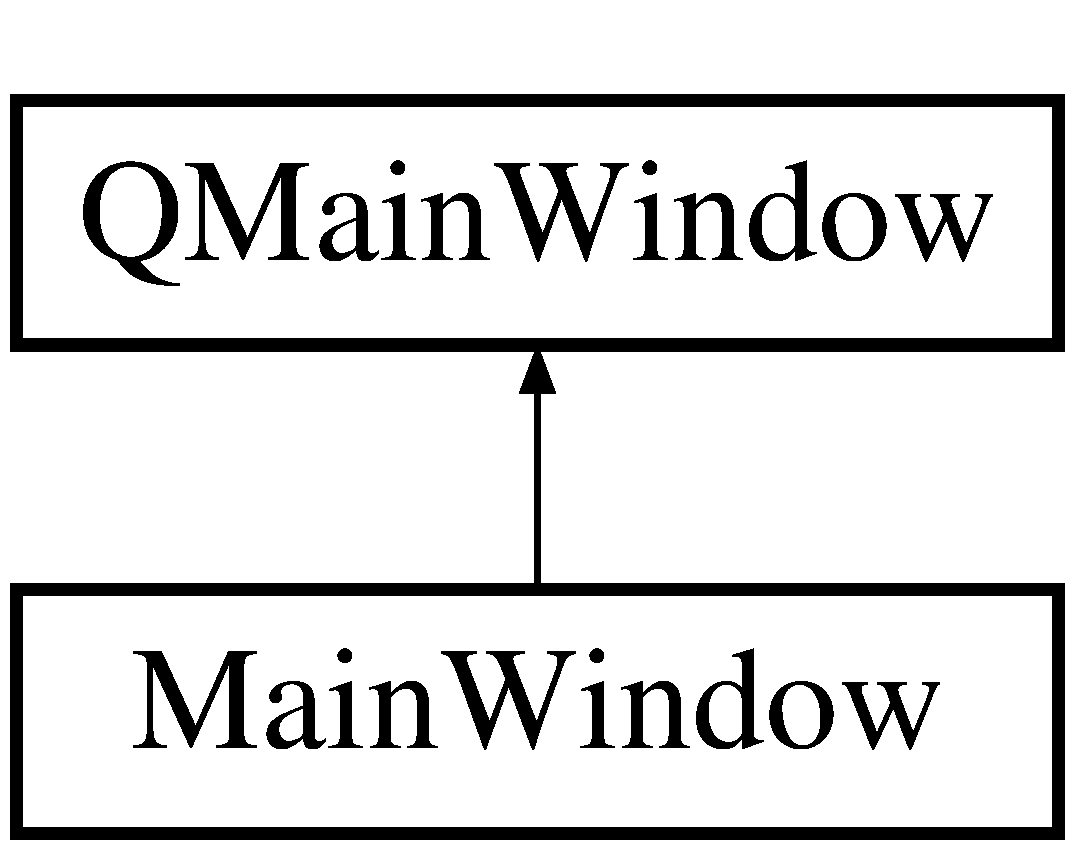
\includegraphics[height=2.000000cm]{class_main_window}
\end{center}
\end{figure}
\subsection*{Public Member Functions}
\begin{DoxyCompactItemize}
\item 
\mbox{\Hypertarget{class_main_window_a8b244be8b7b7db1b08de2a2acb9409db}\label{class_main_window_a8b244be8b7b7db1b08de2a2acb9409db}} 
{\bfseries Main\+Window} (Q\+Widget $\ast$parent=0)
\item 
\mbox{\Hypertarget{class_main_window_a9c4f542263838b9ecd06eae839a42a34}\label{class_main_window_a9c4f542263838b9ecd06eae839a42a34}} 
void {\bfseries key\+Press\+Event} (Q\+Key\+Event $\ast$event)
\end{DoxyCompactItemize}


The documentation for this class was generated from the following files\+:\begin{DoxyCompactItemize}
\item 
D\+:/\+Travail\+Etudiant/fise2-\/sem2/\+Q\+T\+Creator/\+Developpement projet/\+Casse-\/\+Brique/\+Breakout/mainwindow.\+h\item 
D\+:/\+Travail\+Etudiant/fise2-\/sem2/\+Q\+T\+Creator/\+Developpement projet/\+Casse-\/\+Brique/\+Breakout/mainwindow.\+cpp\end{DoxyCompactItemize}

\hypertarget{class_my_g_l_widget}{}\section{My\+G\+L\+Widget Class Reference}
\label{class_my_g_l_widget}\index{My\+G\+L\+Widget@{My\+G\+L\+Widget}}
Inheritance diagram for My\+G\+L\+Widget\+:\begin{figure}[H]
\begin{center}
\leavevmode
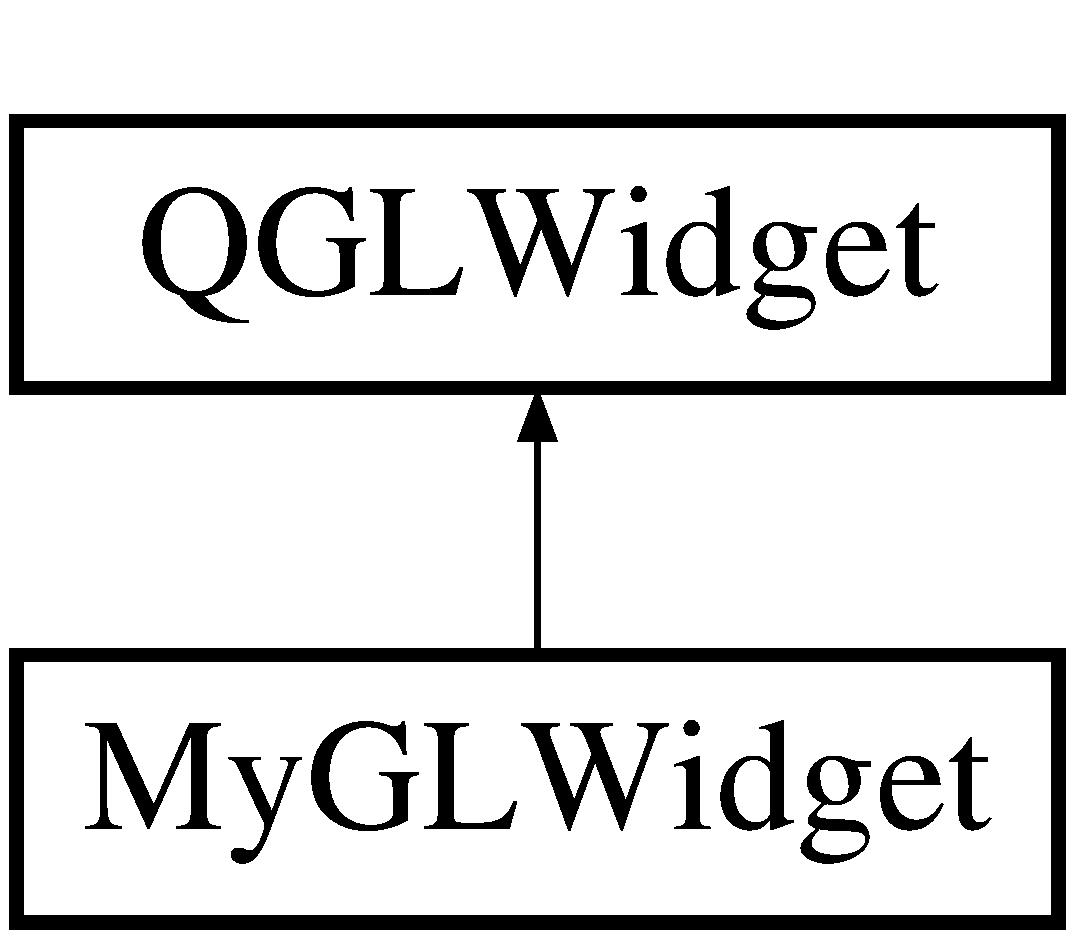
\includegraphics[height=2.000000cm]{class_my_g_l_widget}
\end{center}
\end{figure}
\subsection*{Public Member Functions}
\begin{DoxyCompactItemize}
\item 
\mbox{\Hypertarget{class_my_g_l_widget_a50dfc5ed9f6874956b09378e82265fda}\label{class_my_g_l_widget_a50dfc5ed9f6874956b09378e82265fda}} 
{\bfseries My\+G\+L\+Widget} (Q\+Widget $\ast$parent=nullptr)
\item 
\mbox{\Hypertarget{class_my_g_l_widget_a519efceb466527b8730d82ee1a0da8fb}\label{class_my_g_l_widget_a519efceb466527b8730d82ee1a0da8fb}} 
void {\bfseries mouse\+Move\+Event} (Q\+Mouse\+Event $\ast$event)
\item 
\mbox{\Hypertarget{class_my_g_l_widget_a3e963e10932c45bd4f95813bfa533bfc}\label{class_my_g_l_widget_a3e963e10932c45bd4f95813bfa533bfc}} 
void {\bfseries update\+Cam\+Move\+Event} (int vectX, int vectY)
\end{DoxyCompactItemize}
\subsection*{Public Attributes}
\begin{DoxyCompactItemize}
\item 
\mbox{\Hypertarget{class_my_g_l_widget_a10b11952a864dfa4827c97039f3313bf}\label{class_my_g_l_widget_a10b11952a864dfa4827c97039f3313bf}} 
\mbox{\hyperlink{class_game_manager}{Game\+Manager}} {\bfseries game}
\end{DoxyCompactItemize}
\subsection*{Protected Member Functions}
\begin{DoxyCompactItemize}
\item 
\mbox{\Hypertarget{class_my_g_l_widget_a5c536c2ebab76533eb16eac0a9830c8e}\label{class_my_g_l_widget_a5c536c2ebab76533eb16eac0a9830c8e}} 
void {\bfseries initialize\+GL} ()
\item 
\mbox{\Hypertarget{class_my_g_l_widget_a9717968e75b8a7fc358b947f31eb2690}\label{class_my_g_l_widget_a9717968e75b8a7fc358b947f31eb2690}} 
void {\bfseries resize\+GL} (int width, int height)
\item 
\mbox{\Hypertarget{class_my_g_l_widget_ad0e4171fab09ad54d4e2d23e7d6541eb}\label{class_my_g_l_widget_ad0e4171fab09ad54d4e2d23e7d6541eb}} 
void {\bfseries paint\+GL} ()
\item 
\mbox{\Hypertarget{class_my_g_l_widget_a170905e3688320a2286d3c19a3c4d83a}\label{class_my_g_l_widget_a170905e3688320a2286d3c19a3c4d83a}} 
void {\bfseries draw\+Ball} ()
\item 
\mbox{\Hypertarget{class_my_g_l_widget_a895664084af28911b896b43335da71d0}\label{class_my_g_l_widget_a895664084af28911b896b43335da71d0}} 
void {\bfseries draw\+Pallet} ()
\item 
\mbox{\Hypertarget{class_my_g_l_widget_a493775e718c254eb669f75548eb7d870}\label{class_my_g_l_widget_a493775e718c254eb669f75548eb7d870}} 
void {\bfseries dessine\+Cube} (double centerX, double centerY, double centerZ, double width, double height, int lp\+Tot, int lp)
\end{DoxyCompactItemize}


The documentation for this class was generated from the following files\+:\begin{DoxyCompactItemize}
\item 
D\+:/\+Travail\+Etudiant/fise2-\/sem2/\+Q\+T\+Creator/\+Developpement projet/\+Casse-\/\+Brique/\+Breakout/myglwidget.\+h\item 
D\+:/\+Travail\+Etudiant/fise2-\/sem2/\+Q\+T\+Creator/\+Developpement projet/\+Casse-\/\+Brique/\+Breakout/myglwidget.\+cpp\end{DoxyCompactItemize}

\hypertarget{class_open_cv_widget}{}\section{Open\+Cv\+Widget Class Reference}
\label{class_open_cv_widget}\index{Open\+Cv\+Widget@{Open\+Cv\+Widget}}
\subsection*{Public Attributes}
\begin{DoxyCompactItemize}
\item 
\mbox{\Hypertarget{class_open_cv_widget_a95a6faa37072434e852d626f0a3ee5a9}\label{class_open_cv_widget_a95a6faa37072434e852d626f0a3ee5a9}} 
int {\bfseries frame\+Width}
\item 
\mbox{\Hypertarget{class_open_cv_widget_a5dd41b76affe4c4a37b9502bf7ed9dda}\label{class_open_cv_widget_a5dd41b76affe4c4a37b9502bf7ed9dda}} 
int {\bfseries frame\+Height}
\item 
\mbox{\Hypertarget{class_open_cv_widget_aedde6affb6c0d453f563195013800d9e}\label{class_open_cv_widget_aedde6affb6c0d453f563195013800d9e}} 
int {\bfseries sub\+Image\+Width}
\item 
\mbox{\Hypertarget{class_open_cv_widget_a6cb6b03a5d6ef68a55ff2aaae6a12465}\label{class_open_cv_widget_a6cb6b03a5d6ef68a55ff2aaae6a12465}} 
int {\bfseries sub\+Image\+Height}
\item 
\mbox{\Hypertarget{class_open_cv_widget_abcfddda69b2bc5752751d8df8ee27691}\label{class_open_cv_widget_abcfddda69b2bc5752751d8df8ee27691}} 
int {\bfseries template\+Width}
\item 
\mbox{\Hypertarget{class_open_cv_widget_a2d3122dccb9094d5fea1ca8bbc439954}\label{class_open_cv_widget_a2d3122dccb9094d5fea1ca8bbc439954}} 
int {\bfseries template\+Height}
\item 
\mbox{\Hypertarget{class_open_cv_widget_aa241205fdfbc332e7bc40974a4bc5667}\label{class_open_cv_widget_aa241205fdfbc332e7bc40974a4bc5667}} 
bool {\bfseries state}
\item 
\mbox{\Hypertarget{class_open_cv_widget_ad0cb1cbe57dd17e340461a6f60f743cf}\label{class_open_cv_widget_ad0cb1cbe57dd17e340461a6f60f743cf}} 
Rect {\bfseries working\+Rect\+\_\+}
\item 
\mbox{\Hypertarget{class_open_cv_widget_a81c8a710b09fa082c8288f5781030fb0}\label{class_open_cv_widget_a81c8a710b09fa082c8288f5781030fb0}} 
Rect {\bfseries template\+Rect\+\_\+}
\item 
\mbox{\Hypertarget{class_open_cv_widget_aaf9445696f65d650ae8ee576dc303eaf}\label{class_open_cv_widget_aaf9445696f65d650ae8ee576dc303eaf}} 
Point {\bfseries working\+Center\+\_\+}
\item 
\mbox{\Hypertarget{class_open_cv_widget_a1ede2abdfc5042232566cb2eec7844ee}\label{class_open_cv_widget_a1ede2abdfc5042232566cb2eec7844ee}} 
Video\+Capture {\bfseries cap}
\end{DoxyCompactItemize}


The documentation for this class was generated from the following files\+:\begin{DoxyCompactItemize}
\item 
D\+:/\+Travail\+Etudiant/fise2-\/sem2/\+Q\+T\+Creator/\+Developpement projet/\+Casse-\/\+Brique/\+Breakout/opencvwidget.\+h\item 
D\+:/\+Travail\+Etudiant/fise2-\/sem2/\+Q\+T\+Creator/\+Developpement projet/\+Casse-\/\+Brique/\+Breakout/opencvwidget.\+cpp\end{DoxyCompactItemize}

\hypertarget{class_palette}{}\section{Palette Class Reference}
\label{class_palette}\index{Palette@{Palette}}
Inheritance diagram for Palette\+:\begin{figure}[H]
\begin{center}
\leavevmode
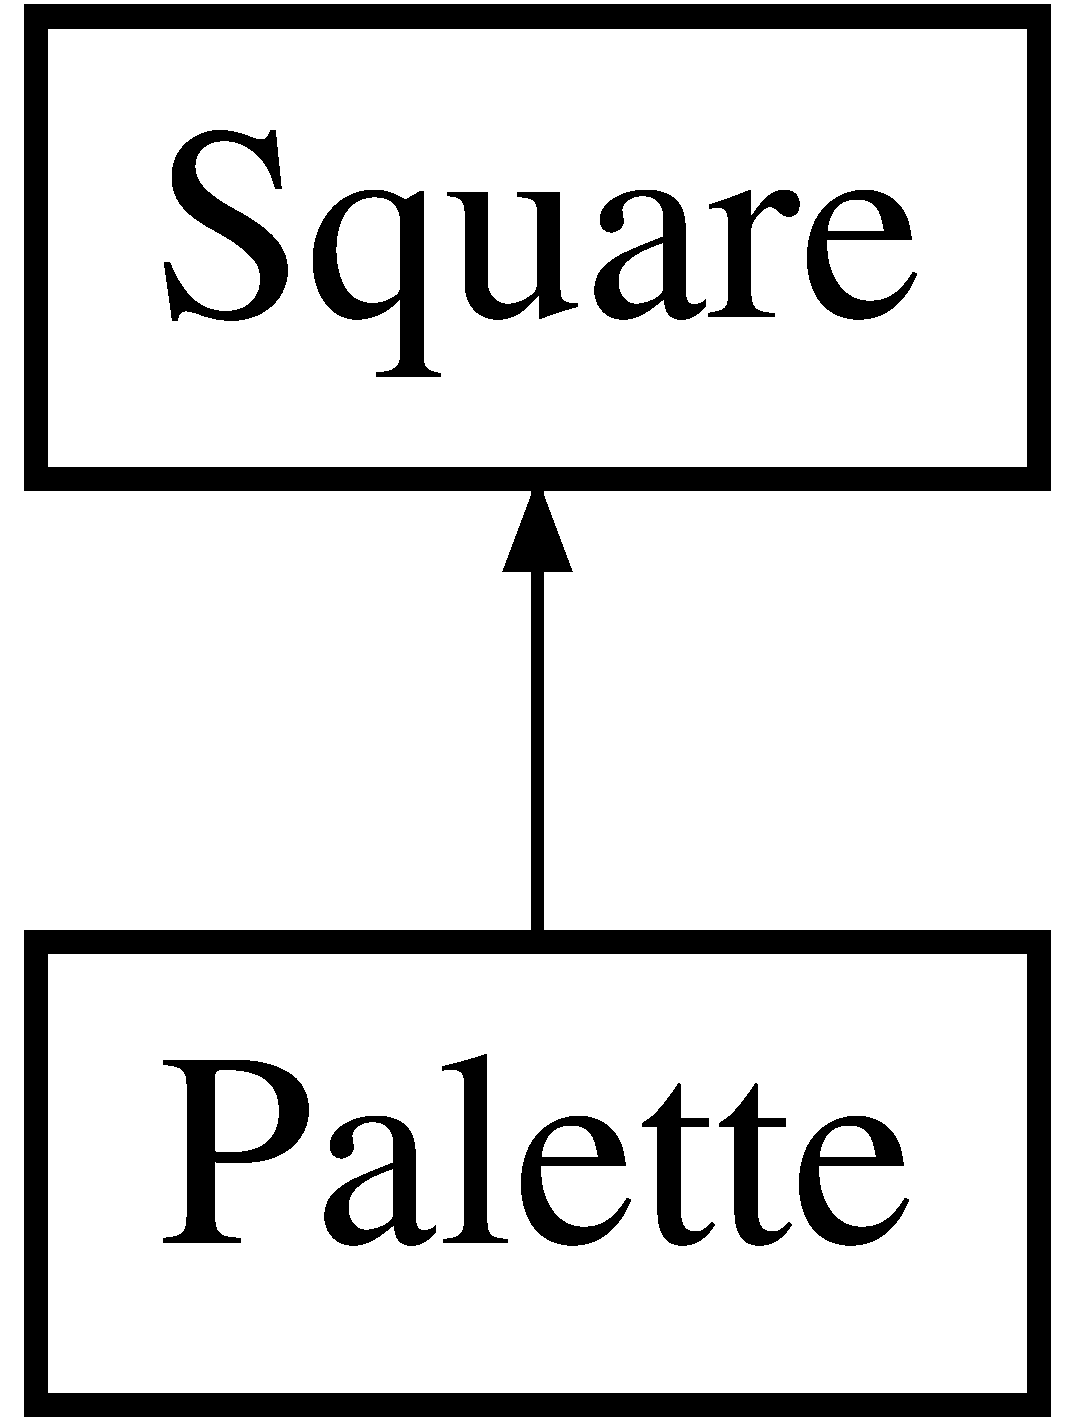
\includegraphics[height=2.000000cm]{class_palette}
\end{center}
\end{figure}
\subsection*{Public Member Functions}
\begin{DoxyCompactItemize}
\item 
\mbox{\Hypertarget{class_palette_aba73583ea3ed774a01dc91768c06b136}\label{class_palette_aba73583ea3ed774a01dc91768c06b136}} 
{\bfseries Palette} (double width, double height, double x, double y, double z, double speed)
\item 
\mbox{\Hypertarget{class_palette_a3668970bbba4c28104443ff68a682da9}\label{class_palette_a3668970bbba4c28104443ff68a682da9}} 
double {\bfseries get\+Speed} ()
\item 
\mbox{\Hypertarget{class_palette_ad8d5e54600152a30732b766f8a1d7739}\label{class_palette_ad8d5e54600152a30732b766f8a1d7739}} 
void {\bfseries set\+Speed} (double sp)
\end{DoxyCompactItemize}


The documentation for this class was generated from the following files\+:\begin{DoxyCompactItemize}
\item 
D\+:/\+Travail\+Etudiant/fise2-\/sem2/\+Q\+T\+Creator/\+Developpement projet/\+Casse-\/\+Brique/\+Breakout/palette.\+h\item 
D\+:/\+Travail\+Etudiant/fise2-\/sem2/\+Q\+T\+Creator/\+Developpement projet/\+Casse-\/\+Brique/\+Breakout/palette.\+cpp\end{DoxyCompactItemize}

\hypertarget{class_player}{}\section{Player Class Reference}
\label{class_player}\index{Player@{Player}}
\subsection*{Public Member Functions}
\begin{DoxyCompactItemize}
\item 
\mbox{\Hypertarget{class_player_adf2e45581d8fd61e26328fa48d13b9b7}\label{class_player_adf2e45581d8fd61e26328fa48d13b9b7}} 
{\bfseries Player} (const \mbox{\hyperlink{class_player}{Player}} \&p)
\item 
\mbox{\Hypertarget{class_player_ac3ad5e51b95a604a27c6f8ac6ecc6f90}\label{class_player_ac3ad5e51b95a604a27c6f8ac6ecc6f90}} 
int {\bfseries get\+Life\+Point} ()
\item 
\mbox{\Hypertarget{class_player_a97e5447778ae6c384eedc532dcd8431d}\label{class_player_a97e5447778ae6c384eedc532dcd8431d}} 
int {\bfseries get\+Score} ()
\item 
\mbox{\Hypertarget{class_player_a23c9b25aeb8dd1ff86d03d993e07a73d}\label{class_player_a23c9b25aeb8dd1ff86d03d993e07a73d}} 
void {\bfseries set\+Score} (int score)
\item 
\mbox{\Hypertarget{class_player_a3fc95cf72792aad03d73c58998ab2643}\label{class_player_a3fc95cf72792aad03d73c58998ab2643}} 
void {\bfseries set\+Life\+Point} (int Life\+Point)
\item 
\mbox{\Hypertarget{class_player_a6072dd0a4fe43d4f4bd418b612c96f7c}\label{class_player_a6072dd0a4fe43d4f4bd418b612c96f7c}} 
void {\bfseries set\+Nb\+Win} (int nb)
\item 
\mbox{\Hypertarget{class_player_aa9728db5b22d438505b4694c5ea03f75}\label{class_player_aa9728db5b22d438505b4694c5ea03f75}} 
void {\bfseries set\+Name} (string name)
\item 
\mbox{\Hypertarget{class_player_af9a6045fa96f736664c4eab4caa5e8e5}\label{class_player_af9a6045fa96f736664c4eab4caa5e8e5}} 
string {\bfseries get\+Name} ()
\item 
\mbox{\Hypertarget{class_player_a47147bc978d0f5e89db3a6c40b9215db}\label{class_player_a47147bc978d0f5e89db3a6c40b9215db}} 
int {\bfseries get\+Nb\+Win} ()
\item 
\mbox{\Hypertarget{class_player_aef7ebb7b9d9e1bd5383f30f74e4accf2}\label{class_player_aef7ebb7b9d9e1bd5383f30f74e4accf2}} 
void {\bfseries charger} (ifstream \&is)
\item 
\mbox{\Hypertarget{class_player_ab5e7a54f06ca7caf4fa48860d67f9dc6}\label{class_player_ab5e7a54f06ca7caf4fa48860d67f9dc6}} 
void {\bfseries sauver} (ofstream \&os)
\item 
\mbox{\Hypertarget{class_player_af1a5f90edb6b0705a4ad4c6d23b79d95}\label{class_player_af1a5f90edb6b0705a4ad4c6d23b79d95}} 
bool {\bfseries operator$<$} (const \mbox{\hyperlink{class_player}{Player}} \&p) const
\end{DoxyCompactItemize}


The documentation for this class was generated from the following files\+:\begin{DoxyCompactItemize}
\item 
D\+:/\+Travail\+Etudiant/fise2-\/sem2/\+Q\+T\+Creator/\+Developpement projet/\+Casse-\/\+Brique/\+Breakout/player.\+h\item 
D\+:/\+Travail\+Etudiant/fise2-\/sem2/\+Q\+T\+Creator/\+Developpement projet/\+Casse-\/\+Brique/\+Breakout/player.\+cpp\end{DoxyCompactItemize}

\hypertarget{class_square}{}\section{Square Class Reference}
\label{class_square}\index{Square@{Square}}
Inheritance diagram for Square\+:\begin{figure}[H]
\begin{center}
\leavevmode
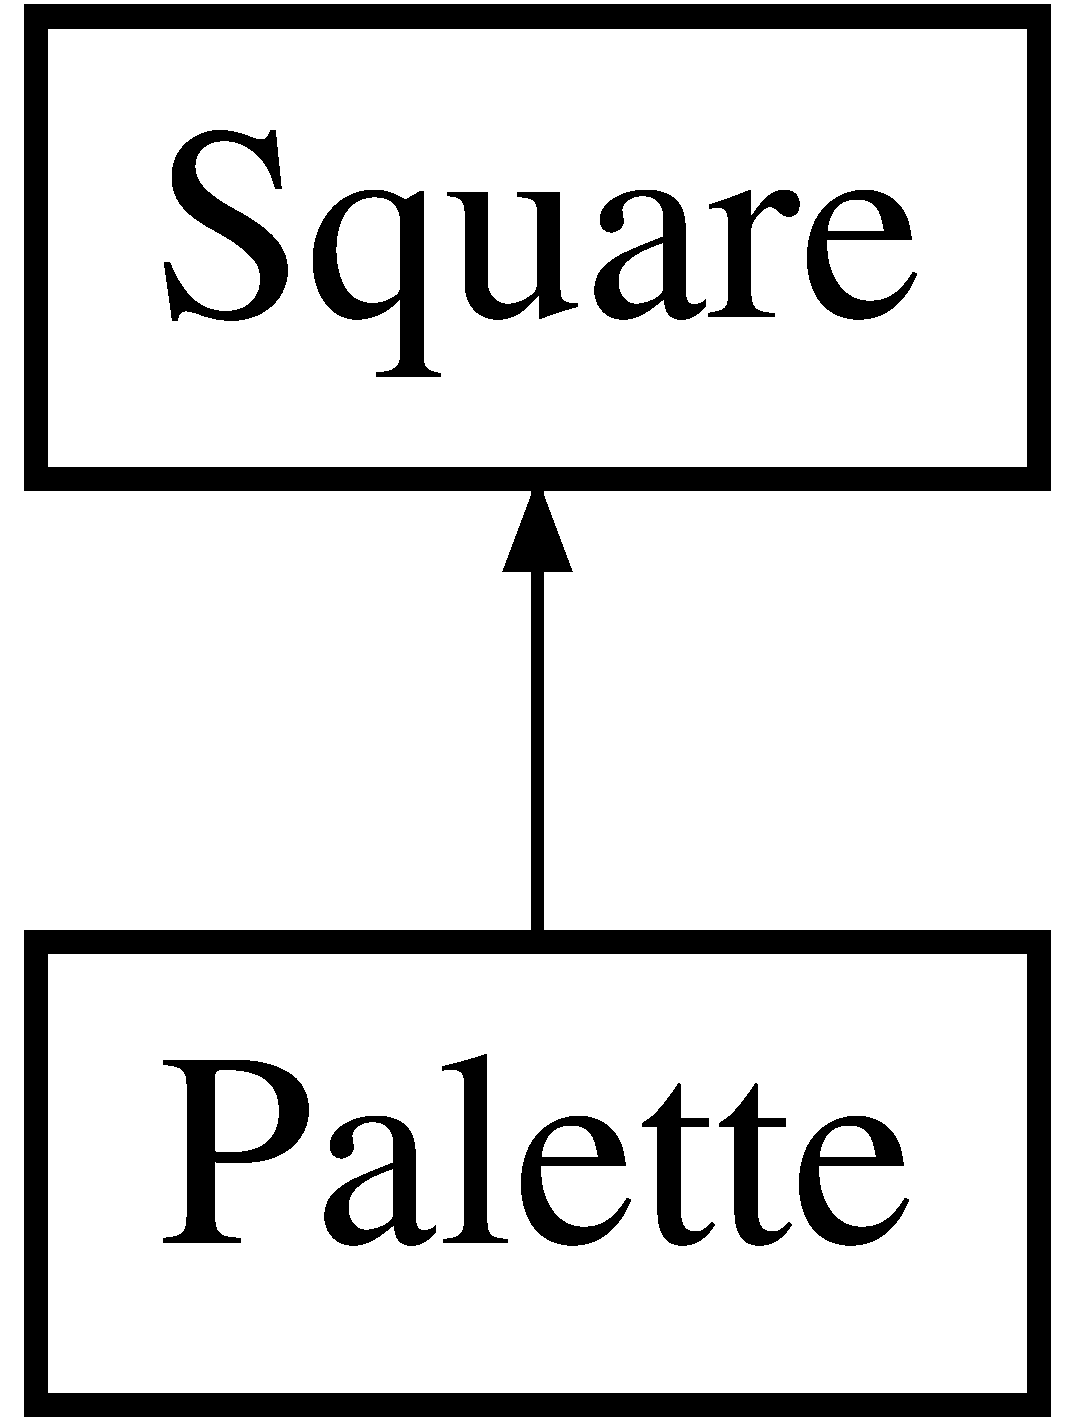
\includegraphics[height=2.000000cm]{class_square}
\end{center}
\end{figure}
\subsection*{Public Member Functions}
\begin{DoxyCompactItemize}
\item 
\mbox{\Hypertarget{class_square_a27551dfdcf961cba100f79bc3441ead3}\label{class_square_a27551dfdcf961cba100f79bc3441ead3}} 
{\bfseries Square} (double width, double height, double X, double Y, double Z, int life)
\item 
\mbox{\Hypertarget{class_square_abca130ad5c32ded493bc56851de84974}\label{class_square_abca130ad5c32ded493bc56851de84974}} 
double {\bfseries getX} ()
\item 
\mbox{\Hypertarget{class_square_a466213e529d0623f27dd59baa5fd425c}\label{class_square_a466213e529d0623f27dd59baa5fd425c}} 
double {\bfseries getY} ()
\item 
\mbox{\Hypertarget{class_square_add85982817300e975f00d982c2944fd3}\label{class_square_add85982817300e975f00d982c2944fd3}} 
double {\bfseries getZ} ()
\item 
\mbox{\Hypertarget{class_square_a5a52ced157d32d3fe038c3674dc7c975}\label{class_square_a5a52ced157d32d3fe038c3674dc7c975}} 
double {\bfseries get\+Score} ()
\item 
\mbox{\Hypertarget{class_square_a3e8803173f2c9c75df15689760a7db68}\label{class_square_a3e8803173f2c9c75df15689760a7db68}} 
double {\bfseries get\+Width} ()
\item 
\mbox{\Hypertarget{class_square_a2759b76cb77ad8310d37e5f8464f6d0f}\label{class_square_a2759b76cb77ad8310d37e5f8464f6d0f}} 
double {\bfseries get\+Height} ()
\item 
\mbox{\Hypertarget{class_square_a8a9dc441b3a1108c52024d5adf25fa80}\label{class_square_a8a9dc441b3a1108c52024d5adf25fa80}} 
int {\bfseries get\+Life} ()
\item 
\mbox{\Hypertarget{class_square_a115fdac881e80628eca323b22d5a0280}\label{class_square_a115fdac881e80628eca323b22d5a0280}} 
void {\bfseries set\+Life} (int life)
\item 
\mbox{\Hypertarget{class_square_a9c14b2ee20078f70e313c1cb62965106}\label{class_square_a9c14b2ee20078f70e313c1cb62965106}} 
void {\bfseries setX} (double X)
\item 
\mbox{\Hypertarget{class_square_a9346b7fc5a92f4ffce92e59d3d9b22b8}\label{class_square_a9346b7fc5a92f4ffce92e59d3d9b22b8}} 
void {\bfseries setY} (double Y)
\item 
\mbox{\Hypertarget{class_square_aa54150595cc276766eab4e251dafd33e}\label{class_square_aa54150595cc276766eab4e251dafd33e}} 
void {\bfseries setZ} (double Z)
\item 
\mbox{\Hypertarget{class_square_ad1d24f2813f78e5052d8085473d222b9}\label{class_square_ad1d24f2813f78e5052d8085473d222b9}} 
void {\bfseries set\+Width} (double width)
\end{DoxyCompactItemize}


The documentation for this class was generated from the following files\+:\begin{DoxyCompactItemize}
\item 
D\+:/\+Travail\+Etudiant/fise2-\/sem2/\+Q\+T\+Creator/\+Developpement projet/\+Casse-\/\+Brique/\+Breakout/square.\+h\item 
D\+:/\+Travail\+Etudiant/fise2-\/sem2/\+Q\+T\+Creator/\+Developpement projet/\+Casse-\/\+Brique/\+Breakout/square.\+cpp\end{DoxyCompactItemize}

\chapter{File Documentation}
\hypertarget{gamemanager_8h}{}\section{D\+:/\+Travail\+Etudiant/fise2-\/sem2/\+Q\+T\+Creator/\+Developpement projet/\+Casse-\/\+Brique/\+Breakout/gamemanager.h File Reference}
\label{gamemanager_8h}\index{D\+:/\+Travail\+Etudiant/fise2-\/sem2/\+Q\+T\+Creator/\+Developpement projet/\+Casse-\/\+Brique/\+Breakout/gamemanager.\+h@{D\+:/\+Travail\+Etudiant/fise2-\/sem2/\+Q\+T\+Creator/\+Developpement projet/\+Casse-\/\+Brique/\+Breakout/gamemanager.\+h}}


Gestionnaire de Jeu.  


{\ttfamily \#include \char`\"{}ball.\+h\char`\"{}}\newline
{\ttfamily \#include \char`\"{}square.\+h\char`\"{}}\newline
{\ttfamily \#include \char`\"{}palette.\+h\char`\"{}}\newline
{\ttfamily \#include \char`\"{}player.\+h\char`\"{}}\newline
{\ttfamily \#include $<$Q\+Point$>$}\newline
\subsection*{Classes}
\begin{DoxyCompactItemize}
\item 
class \mbox{\hyperlink{class_game_manager}{Game\+Manager}}
\begin{DoxyCompactList}\small\item\em Classe regroupant et gérant les éléments du jeu. \end{DoxyCompactList}\end{DoxyCompactItemize}


\subsection{Detailed Description}
Gestionnaire de Jeu. 

\begin{DoxyAuthor}{Author}
Rouby Terenui 
\end{DoxyAuthor}

%--- End generated contents ---

% Index
\backmatter
\newpage
\phantomsection
\clearemptydoublepage
\addcontentsline{toc}{chapter}{Index}
\printindex

\end{document}
